
\begin {document}

\title{CTC/Office User Manual}
\author {Writen by: Christen Reinbeck}
\date{}

\maketitle

\section{CTC}

\subsection{UI Layout}

\begin{figure}[h!]
	\center
	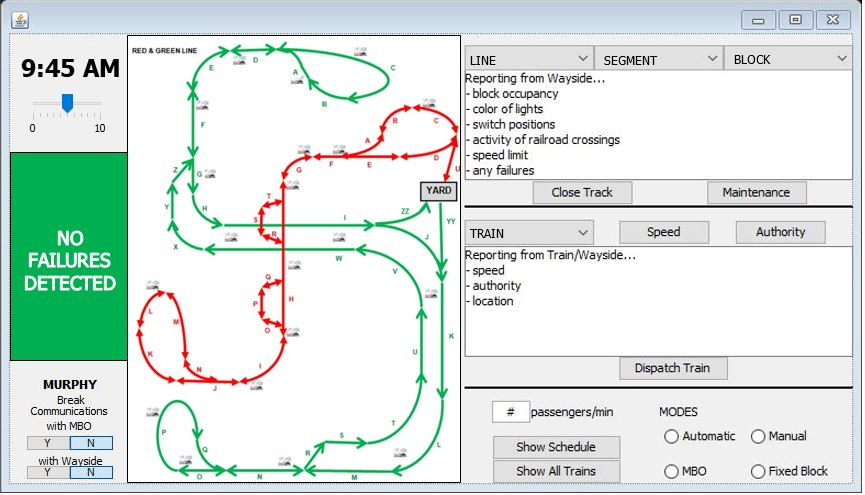
\includegraphics[width=16cm]{CTC_gui}
	\caption{Graphical User Interface for the CTC}
\end{figure}

\subsection{UI Buttons and Actions}
	
	\subsubsection{Time/Fast-Forward Capability}
		\begin{itemize}
			\item Slider – used to control speed of time passing, either regular speed or 10x speed.
			\item Clock – displays time in whatever speed is selected.
		\end{itemize}

	\subsubsection{Failure Detection Sidebar}
		\begin{itemize}
			\item Sidebar color change block – sidebar will display in one of two ways:
				\begin{itemize}	
					\itemo	Green – no failures detected
					\itemo	Red – Failure detected as well as in which line/segment/block
				\end{itemize}
		\end{itemize}

	\subsubsection{Murphy}
		\begin{itemize}
			\item Slider buttons – ability to activate communication breaks between either MBO or Wayside controller for testing purposes.
		\end{itemize}

	\subsubsection{Line Map}
		\begin{itemize}
			\item Displays all sections and lines of the map/system you are currently working on.
		\end{itemize}

	\subsubsection{Block Controls}
		\begin{itemize}
			\item Dropdowns – used to select appropriate line/segment/block that you wish to use.
			\item Text display – displays information as pulled from wayside controller, such as block occupancy, switch status, light color and status, activity of railroad crossings, and block failures.
			\item Close track button – propagates a popup window that restates which block of track you wish to close with either the option to close track or cancel.
			\item Send maintenance button – propagates a popup window that restates which block of track you wish to send maintenance to, with either the option to send or cancel.
		\end{itemize}

	\subsubsection{Train Controls}
		\begin{itemize}
			\item Dropdown – used to select a specific train.
			\item Speed and Authority Buttons – propagates popup windows where you can set speed or authority for a given train.
			\item Text display – displays the current speed and authority of the selected train, and updates should the user change the speed and authority at a given time.
			\item Dispatch train button – propagates a popup window which allows you to dispatch a train from the yard, selecting line, station to go to, speed and authority.
		\end{itemize}

	\subsubsection{Miscellaneous Controls/Info}
		\begin{itemize}
			\item Throughput display – displays number of passengers/hour of the system as a whole.
			\item Show schedule button – propagates a popup window of train schedules from the MBO/Scheduler.
			\item Show all trains button – propagates a popup window of all trains currently dispatched as well as their current GPS location, line, segment, block.
			\item Mode Options for Schedule via radio buttons:
				\begin{itemize}
					\item Automatic – this mode gives the dispatcher two options
						\begin{itemize}
							\item MBO – gets a schedule from the MBO/Scheduler that is most optimized with more trains running.
							\item Fixed Block – also gets a schedule from the MBO/Scheduler but only allows one train/block at any given time.
						\end{itemize}
					\item Manual – dispatcher manually dispatches trains using the aforementioned button.
				\end{itemize}
		\end{itemize}


\end{document}